This section begins with a subsection \Sec{backgr} which places the \nep \ project in the global context.
The following subsections \Sec{spem} and \Sec{hilevel} review more local UKAEA activities 
prior to commencement of \nep, and its concluding subsection brings history up-to-date with
a summary of \nep \ Y1 activities. Much of the material in this \Sec{intro} bears on the choices
made for the Y2 programme discussed in \Sec{taskwork} and summarised in \Sec{summ}.

\subsection{Background}\label{sec:backgr}

In the past few years, the focus of the UKAEA fusion programme has been increasingly
directed towards the design of power-generating reactors, see eg.\ papers presented
at a Royal Sociey meeting in~2018 ``Fusion energy using tokamaks: can development be accelerated?',
notably refs~\cite{Wi19impa, Su19Engi}.
At the start of November~2018, two documents of worldwide importance for the development
of fusion appeared, namely the ITER Research Plan~\cite{iterrp} and the updated
European Research Roadmap~\cite{rdmap}. They correctly emphasise the importance
of modelling \emph{in silico} but are lacking in detail as to how accurate and reliable
models are to be developed in timely fashion for the designers and operators of ITER and DEMO devices.
For example there is lack of usage of the word ``software", implying absence
of the term ``software engineering"(SWEng). However, the increased stress on model
reliability for ``digital twinning" might a priori be expected to require careful management 
of software throughout its entire life-cycle.
%\begin{figure}[h]
%\centerline{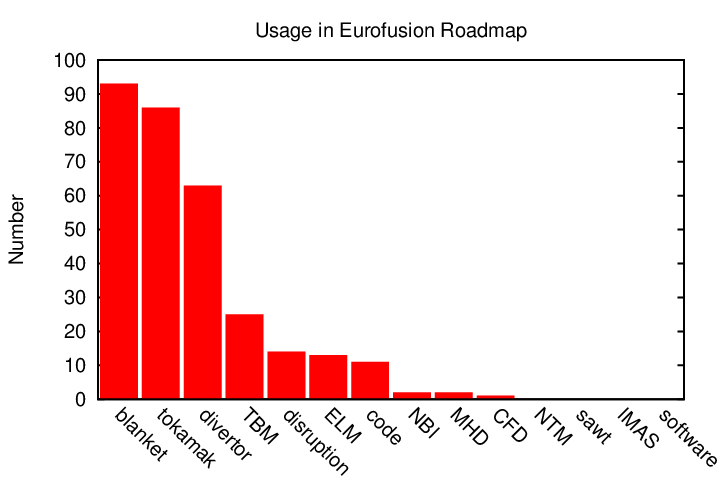
\includegraphics[width=13.0cm]{../png/rdmapw.png}}
%\centerline{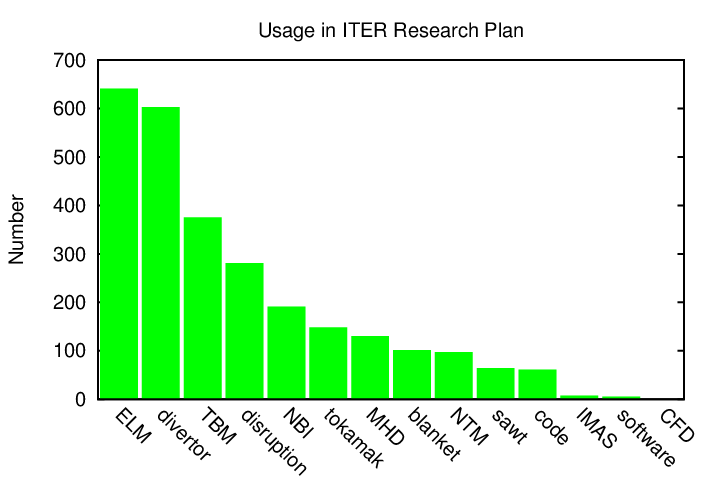
\includegraphics[width=13.0cm]{../png/iterw.png}}
%\caption{Frequency of usage of words/acronyms by refs~\cite{iterrp,rdmap}.
%Analysis by conversion of pdf to text of approx 80 chars/line, counts are number of lines containing
%the word or acronym, count for word ``code" corrected for alternative usage meaning
%``international standard".
%\label{fig:nosw}}
%\end{figure}

There are special features for the software engineer to account for
in a leading-edge technology programme such as fusion reactor 
development, which is nonetheless long-term.  Digitally twinned software must be flexible, 
to deal with issues which perhaps were not initially regarded as important and may require
rapid resolution, for example in the light of new experimental data
or during construction work. This amounts to a requirement that the
software, based on current fusion timelines needs to remain not only usable but
modifiable, perhaps drastically, over at least the next $30$~years needed to see DEMO
into power production.

Concerning existing software, especially for plasma physics modelling, it can be argued that 
the finite difference software (fd) presently underlying much design work is obsolescent in the above
special software engineering terms, being expensive and/or error-prone to maintain as the products of an era when
SWEng was in its infancy. Specifically here is being considered the Patankar scheme~\cite{patankar}
that underlies the SOLPS fluid code known as~B2~\cite[\S\,6]{braams}. SOLPS is for many people
the `gold standard' edge modelling code because it incorporates more physical effects than
more recent developments.
From a practical point-of-view, fd is unsatisfactory for design work because it
fails to give robust error estimates, and inefficient because of
21st Century trends in computer architecture. %, see \Sec{fdiff} for further details.
Typically these schemes are not very accurate with errors of $1$\,\% rising locally to~$10$\,\%.
Recent developments of the \emph{chebfun} approach by Trefethen and co-workers (eg. \ ref~\cite{To15Cont,Ha17Cheb})
are producing
commodity software capable of solving PDEs to `spectral' accuracy in double precision.
Sustained progress here will render these plasma physics' low-order-accurate fd schemes an embarrassment.
There is perhaps an even more significant issue for the use of the particle-based
methods described in say the review~\cite{Wa95a}, since these are associated
with relatively large amplitude sampling `noise'.

\subsection{Spectral/hp Element Method}\label{sec:spem}
Two student projects involving the spectral/hp element method for modelling
the tokamak edge were commissioned by UKAEA from 2015 onwards, see ref~\cite{Ca15Appl, bhojwani},
and a number of other interactions took place, notably presentations by Sherwin
the joint author of the textbook~\cite{karniadakissherwin},
and in 2018 by both Sherwin and his former post-doc Moxey. Just prior to
\nep \ commencement, Arter~\cite{Ar19Chal-ppt} gave a 
presentation at the Isaac Newton Institute explaining the desirability of using
spectral elements for tokamak edge modelling.

Spectral element methods~\cite{pozrikidis} are capable of providing usable error
estimates and of exploiting the
developing architecture to ensure maximum use of complex 2-D, 3-D 
and time-dependent physical models expected to be more robust under 
extrapolation to new situations and regimes. Their extreme accuracy much reduces the need for
special physics-dependent coding, suggesting that a near-complete replacement of code essential
for reactor design is feasible, and if carefully managed, such a new development can meet the
demanding SWEng requirements of the fusion programme.

Amongst spectral element approaches, none has the maturity and the full
range of advantages presented by spectral/hp element. The spectral/hp element method 
(see $650$-page textbook~\cite{karniadakissherwin}) was developed jointly by Karniadakis and Sherwin around the
turn of the Century. In the name, the ``h" implies variable element size, and
``p" implies use of a $p^{th}$-order accurate approximation, where $p$ is an arbitrarily large order.
``Spectral" reinforces the notion that as $p\longrightarrow\infty$, spectral accuracy, ie.\
error smaller than any power of element size, is achievable. This is to be compared with
commercial packages for comparable problems which use low order finite elements, often
restricted to first or second order.
The name spectral/hp does not exclude use also of $r$-refinement, ie.\ elements
moving dynamically better to capture intensifying gradients of say a fluid flow-field.


\Fig{nekhist} indicates the increasing application of the method in published papers to a 
wide range of problems. In addition, there has been commercially driven application of spectral/hp element
to the design of F-1 cars. Other 21st Century developments have seen the
the incorporation of special, geometrically accurate meshing techniques~\cite{Tu17fram} 
into the NekMesh library, which overcome the often large
errors associated with common triangulations of geometry~\cite{Bo12Infl}, and 
production of the Nektar++ library~\cite{Ca15Nekt}.
Further investigation of geometry representation for \nep \ application
is to be found in the Milestone Report~\cite{y1re211}.
\Fig{nekhist} indicates that the latter
has facilitated widespread uptake of the method, giving evidence for a
growing community with large range of applications, many of direct interest to fusion.
\begin{figure}[h]
\centerline{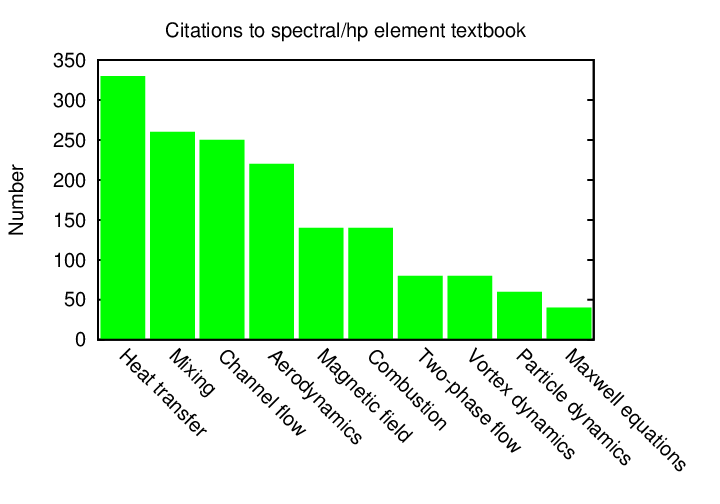
\includegraphics[width=13.0cm]{../png/nektxt.png}}
\centerline{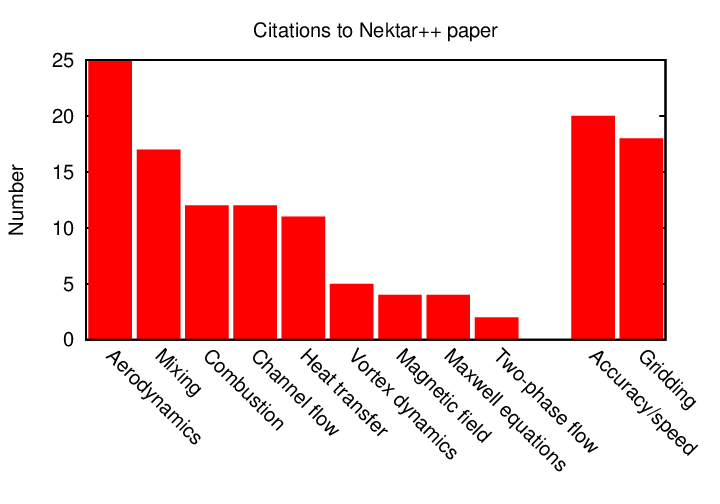
\includegraphics[width=13.0cm]{../png/nektar.png}}
\caption{
Citation counts for applications of the spectral/hp element textbook and Nektar++ library.
Search performed on google scholar(1/5/18) for keywords indicated.
Spectral/hp element textbook from 1997/2003 has 2300 citations, Nektar++ library
description paper from July 2015 has 120 citations (151 as of 1/11/18).
\label{fig:nekhist}}
\end{figure}

The controllable accuracy of spectral element schemes is important despite the inevitable
errors in any experimental confrontation with reality, because of  great advances in techniques 
for fitting models to data, in fields such as optimisation, uncertainty 
quantification and data assimilation, now often bracketed as Machine 
Learning, see recent work by Arter and students~\cite{Ca18Sens,Ar18Data}. 
These advances in VVUQ techniques give more robust fitting with improved error estimates.

One advantage of extreme accuracy that is highlighted here, because of its relevance to the serious
problem of heat deposition on first wall, occurs when there is very anisotropic heat transport,
found in some layered materials or as here, because of a large-scale magnetic field.
If the numerical grid is not aligned with the field, then heat leaks in the normal direction at
every timestep at a rate proportional to cell-size~$h$, leading to an effective heat diffusivity
$D_{\perp,num}\propto h^2/\Delta t$ ($\Delta t$ is time-step size)
which may greatly exceed the intended perpendicular transport.
Even if the grid is field-aligned, either by special local construction or by use of an unstructured, finite element
representation, since a good first wall power distribution requires almost tangential 
incidence,  there will be elements with very small angles leading to poor convergence
properties for most solvers.
However, as \Fig{aniso} shows, for spectral elements,
the effective relative heat diffusivity
remains small over the whole range of~$\phi$, even having a
local minimum at the angle of maximum misalignment.
\begin{figure}[h]
\centerline{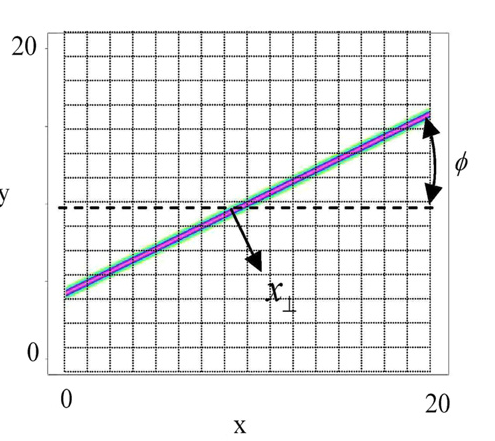
\includegraphics[width=7.0cm]{../png/dirn.png}}
\centerline{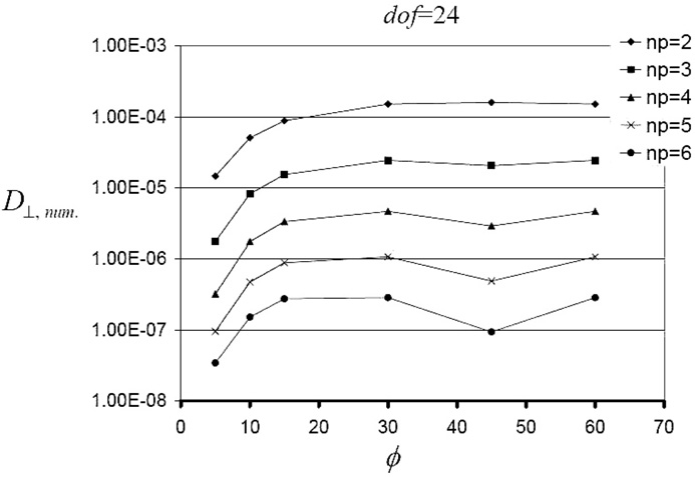
\includegraphics[width=13.0cm]{../png/dirdifus.png}}
\caption{Spectral element methods can model the entire range of misalignment
angles~$\phi$ without any special treatment,
from ref~\protect\cite{Me10Spec}. Figure at top indicates the field direction
relative to the fe mesh,
in the graph below $np$ corresponds to
the order~$p$ and $dof$ to the number of degrees of freedom per unit length.
\label{fig:aniso}}
\end{figure}

\subsection{High Level Integration}\label{sec:hilevel}
Work by Arter, see for example~\cite{Ar18Reac-ppt} 
examined how by use of appropriate software technology, spectral
element software could be integrated into  an object-oriented approach permitting
easy integration into the overall reactor design package.
This is a two-way process, in that design can only proceed at an acceptable
speed using surrogates for full 3-D to 6-D models even on multi-core desktops,
whereas as in critical cases, 3-D to 6-D models may need to be invoked to
reduce uncertainty. Preliminary indications were that this should be achievable
using a graph-based approach, implemented in matrix form, see \Fig{matrixcode}.
\begin{figure}[h]
\centerline{{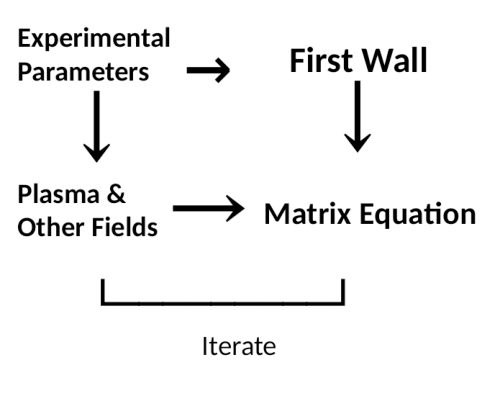
\includegraphics[width=8.0cm]{../png/matrixcode.png}}
}
\caption{Schematic of top-level algorithm.
\label{fig:matrixcode}}
\end{figure}
A bundled capability for producing surrogates needs to be included, and
emphasis needs to be placed upon generating well-documented arms-length interfaces that
can be used by external packages. The programming style described by Arter
et al~\cite{fprog} is particularly appropriate to this purposes, and should be
applicable in any object-oriented language.
There will also be a need for an easy way to specify scalar and vector differentiation
operators.

\subsection{UKAEA Activities to date}\label{sec:todate}
Work to-date on the \nep \ project has been driven by the above considerations. 
Of all the tokamak modelling codes, SOLPS is the one of which development has
been most weighed down by its history, making edge modelling the prime candidate area
for producing new software. The EUROfusion Theory and Advanced Simulation Coordination (E-TASC)
has also recognised this, in that two of the first TSVV
(Theory, Simulation, Verification, and Validation) tasks are to pilot writing of
the European Boundary Code~(EBC), and to launch a major upgrade of the SOLPS
particle code known as EIRENE. These pilot tasks are due to finish at the end of 2020,
and particularly the EBC project has a challenging target to produce significant 
novel physics results, in order to ensure funding for the proposed $5$-year follow-up.

It has been decided  that \nep \ will coordinate primarily with the TSVV EBC project
(which necessarily has to coordinate with the particle code project).
UKAEA staff working on \nep \ have attended the two major meetings of the EBC pilot
phase, and relevant outcomes are discussed in the Milestone Report~\cite{y1re331}.
As pointed out at the meeting by UKAEA staff, some decisions taken to ensure
the EBC targets are met are sub-optimal for a longer term project such as \nep,
never mind a thirty-year horizon.

\nep \ also has to meet other UK SPF aims, based around the four pillars. However,
it seems \nep \ can coordinate with EBC to the extent that it looks to examine a common 2-D~fluid
model in Y3, so that where \nep \ Y2~research tasks are directed towards this same model,
\nep \ should be able to assist EBC with any problems encountered related to those tasks.
Most other research, such as interface design, integration with particle methods etc. \ to
be performed under \nep, should be complementary to the EBC pilot phase development,
and of immense value to a $5$-year follow-on programme.

Other UKAEA activities have been to hold an internal workshop for requirements capture
and an external workshop, which are reported upon in ref~\cite{y1re111a,y1re111b}. 
The above activities have been accompanied by and to some extent driven 
identification and preliminary investigation of the critical research needed
into the physical model, numerical algorithms and software engineering.

Further investigation of particle methods for \nep \ application
is to be found in the Milestone Report~\cite{y1re231}.

%
%Research will indicate whether the approach adopted by BOUT++~\cite{Du13BOUT}
%or that of the spectral method-based project Dedalus (http://dedalus-project.org/)
%is more appropriate, possibly a combination of the two will be found optimum.
%
%\clearpage
%\input{fdiff}
%
%
